\documentclass[12pt,a4paper]{article}
\usepackage[utf8]{inputenc}
\usepackage{amsmath}
\usepackage{amsfonts}
\usepackage{amssymb}
\usepackage{graphicx}
\usepackage{algorithm}
\usepackage{algorithmic}
\usepackage{tikz}
\usepackage{xcolor}
\usepackage{hyperref}
\usepackage{listings}
\usepackage{float}
\usepackage{subcaption}

\usetikzlibrary{arrows.meta, positioning, shapes.geometric}

\title{Sumatra's Bang-Bang Trajectory Planning System\\
\large A Comprehensive Guide to Time-Optimal Robot Motion}
\author{Analysis Document\\TIGERs Mannheim RoboCup SSL Team}
\date{\today}

\begin{document}

\maketitle
\tableofcontents
\newpage

\section{Introduction: What is Trajectory Planning?}

Imagine you're driving a car and you need to get from point A to point B as quickly as possible. You have two constraints:
\begin{itemize}
    \item Maximum speed limit (you can't go faster than 100 km/h)
    \item Maximum acceleration (your car can't accelerate instantly)
\end{itemize}

The question is: \textbf{What's the fastest way to reach your destination?}

The answer is surprisingly simple: \textbf{Bang-Bang Control}
\begin{enumerate}
    \item \textbf{Bang} - Accelerate at maximum acceleration
    \item \textbf{Bang} - Decelerate at maximum deceleration
\end{enumerate}

This is exactly what Sumatra's trajectory planning system does for robots!

\section{Core Concept: Bang-Bang Control}

\subsection{Why is it called "Bang-Bang"?}

The name comes from control theory. Imagine a light switch - it's either fully ON or fully OFF, never halfway. Similarly, Bang-Bang control uses:
\begin{itemize}
    \item Maximum positive acceleration (full throttle forward)
    \item Maximum negative acceleration (full brakes)
    \item Zero acceleration (cruising at constant speed)
\end{itemize}

\subsection{The Three Trajectory Profiles}

Depending on the distance and initial velocity, Bang-Bang control creates one of three motion profiles:

\subsubsection{1. Triangular Profile (Short Distance)}

When the distance is short, the robot:
\begin{enumerate}
    \item Accelerates at max acceleration
    \item Immediately decelerates at max deceleration (no cruising)
\end{enumerate}

\begin{center}
\begin{tikzpicture}[scale=1.5]
    % Axes
    \draw[->] (0,0) -- (4,0) node[right] {Time};
    \draw[->] (0,0) -- (0,2.5) node[above] {Velocity};
    
    % Triangular velocity profile
    \draw[thick, blue] (0,0) -- (1.5,1.5) -- (3,0);
    \node[below] at (1.5,0) {$t_1$};
    \node[below] at (3,0) {$t_2$};
    \node[right] at (1.5,1.5) {$v_{peak}$};
    
    % Labels
    \node at (0.75,0.5) {Accel};
    \node at (2.25,0.5) {Decel};
\end{tikzpicture}
\end{center}

\textbf{Physics Explanation:}
\begin{align}
    v_{peak} &= \sqrt{a_{max} \cdot d_{total}} \\
    t_{total} &= 2 \cdot \frac{v_{peak}}{a_{max}}
\end{align}

Where:
\begin{itemize}
    \item $v_{peak}$ = Peak velocity reached
    \item $a_{max}$ = Maximum acceleration
    \item $d_{total}$ = Total distance to travel
\end{itemize}

\subsubsection{2. Trapezoidal Profile (Long Distance)}

When the distance is long enough, the robot:
\begin{enumerate}
    \item Accelerates to maximum velocity
    \item Cruises at maximum velocity
    \item Decelerates to stop
\end{enumerate}

\begin{center}
\begin{tikzpicture}[scale=1.5]
    % Axes
    \draw[->] (0,0) -- (5,0) node[right] {Time};
    \draw[->] (0,0) -- (0,2.5) node[above] {Velocity};
    
    % Trapezoidal velocity profile
    \draw[thick, blue] (0,0) -- (1,1.5) -- (3,1.5) -- (4,0);
    \node[below] at (1,0) {$t_1$};
    \node[below] at (3,0) {$t_2$};
    \node[below] at (4,0) {$t_3$};
    \node[right] at (3,1.5) {$v_{max}$};
    
    % Labels
    \node at (0.5,0.5) {Acc};
    \node at (2,1.8) {Cruise};
    \node at (3.5,0.5) {Dec};
\end{tikzpicture}
\end{center}

\textbf{Physics Explanation:}
\begin{align}
    t_{accel} &= \frac{v_{max}}{a_{max}} \\
    d_{accel} &= \frac{1}{2} a_{max} \cdot t_{accel}^2 \\
    d_{cruise} &= d_{total} - 2 \cdot d_{accel} \\
    t_{cruise} &= \frac{d_{cruise}}{v_{max}}
\end{align}

\subsubsection{3. Reverse Profile (Wrong Direction)}

When the robot is initially moving in the wrong direction:
\begin{enumerate}
    \item Decelerate to stop (brake!)
    \item Accelerate in the correct direction
    \item Follow triangular or trapezoidal profile
\end{enumerate}

\section{The Mathematics Behind Bang-Bang Control}

\subsection{Basic Kinematics}

The fundamental equations of motion that govern the trajectory are:

\begin{align}
    \text{Position: } s(t) &= s_0 + v_0 \cdot t + \frac{1}{2} a \cdot t^2 \\
    \text{Velocity: } v(t) &= v_0 + a \cdot t \\
    \text{Acceleration: } a(t) &= \begin{cases}
        +a_{max} & \text{accelerating} \\
        0 & \text{cruising} \\
        -a_{max} & \text{decelerating}
    \end{cases}
\end{align}

\subsection{Determining the Profile Type}

Sumatra's algorithm decides which profile to use based on these calculations:

\begin{algorithm}
\caption{Profile Selection Algorithm}
\begin{algorithmic}
\STATE \textbf{Input:} $s_0$ (initial position), $s_{target}$ (target position), $v_0$ (initial velocity)
\STATE \textbf{Output:} Trajectory profile type

\STATE $d = s_{target} - s_0$ \COMMENT{Distance to travel}
\STATE $s_{brake} = \frac{v_0^2}{2 \cdot a_{max}}$ \COMMENT{Distance needed to stop}

\IF{$s_{brake} > |d|$}
    \STATE \textbf{Return} "Reverse Profile" \COMMENT{Moving too fast in wrong direction}
\ELSE
    \STATE $v_{peak} = \sqrt{v_0^2 + 2 \cdot a_{max} \cdot |d|}$
    \IF{$v_{peak} < v_{max}$}
        \STATE \textbf{Return} "Triangular Profile"
    \ELSE
        \STATE \textbf{Return} "Trapezoidal Profile"
    \ENDIF
\ENDIF
\end{algorithmic}
\end{algorithm}

\section{2D Trajectory Synchronization}

\subsection{The Challenge}

A robot moves in 2D (X and Y directions). We need both axes to finish their trajectories at the same time, otherwise the robot would move in a zigzag pattern!

\begin{figure}[H]
\centering
\begin{tikzpicture}[scale=2]
    % Grid
    \draw[gray, very thin, dashed] (0,0) grid (3,2);
    
    % Axes
    \draw[->] (0,0) -- (3.5,0) node[right] {X};
    \draw[->] (0,0) -- (0,2.5) node[above] {Y};
    
    % Bad trajectory (unsynchronized)
    \draw[red, thick, dashed] (0,0) -- (2.5,0) -- (2.5,1.5);
    \node[red, right] at (2.7,0.7) {Unsynchronized};
    
    % Good trajectory (synchronized)
    \draw[green, thick] (0,0) -- (2.5,1.5);
    \node[green, right] at (2.5,1.5) {Synchronized};
    
    % Start and end points
    \filldraw (0,0) circle (0.05) node[below left] {Start};
    \filldraw (2.5,1.5) circle (0.05) node[above right] {Goal};
\end{tikzpicture}
\caption{Synchronized vs Unsynchronized Trajectories}
\end{figure}

\subsection{The Alpha-Synchronization Algorithm}

Sumatra uses a clever algorithm to synchronize X and Y movements:

\begin{enumerate}
    \item \textbf{Initial Guess:} Start with $\alpha = 45°$ (equal speed distribution)
    \item \textbf{Velocity Distribution:}
    \begin{align}
        v_{max,x} &= v_{max} \cdot \cos(\alpha) \\
        v_{max,y} &= v_{max} \cdot \sin(\alpha) \\
        a_{max,x} &= a_{max} \cdot \cos(\alpha) \\
        a_{max,y} &= a_{max} \cdot \sin(\alpha)
    \end{align}
    
    \item \textbf{Generate Trajectories:} Create 1D trajectories for X and Y
    
    \item \textbf{Check Synchronization:}
    \begin{itemize}
        \item If $t_x > t_y$: Decrease $\alpha$ (give more speed to X)
        \item If $t_y > t_x$: Increase $\alpha$ (give more speed to Y)
    \end{itemize}
    
    \item \textbf{Binary Search:} Repeat until $|t_x - t_y| < \epsilon$ (typically 1ms)
\end{enumerate}

\begin{figure}[H]
\centering
\begin{tikzpicture}[scale=2]
    % Unit circle showing alpha
    \draw[->] (0,0) -- (2,0) node[right] {$v_{max} \cos(\alpha)$};
    \draw[->] (0,0) -- (0,2) node[above] {$v_{max} \sin(\alpha)$};
    
    % Velocity vector
    \draw[->, thick, blue] (0,0) -- (1.414,1.414);
    \draw[dashed] (1.414,0) -- (1.414,1.414);
    \draw[dashed] (0,1.414) -- (1.414,1.414);
    
    % Angle
    \draw (0.3,0) arc (0:45:0.3);
    \node at (0.5,0.2) {$\alpha$};
    
    % Labels
    \node[below] at (1.414,0) {$v_x$};
    \node[left] at (0,1.414) {$v_y$};
    \node[above right] at (1.414,1.414) {$v_{max}$};
\end{tikzpicture}
\caption{Velocity Distribution using Alpha Angle}
\end{figure}

\section{The Curved Path Problem: Bang-Bang's Limitation}

\subsection{Why Bang-Bang Creates Jerky Motion}

Bang-Bang control is mathematically optimal for \textbf{straight-line paths}, but real robot soccer requires navigating around obstacles, which creates curved paths. Here's the fundamental problem:

\begin{figure}[H]
\centering
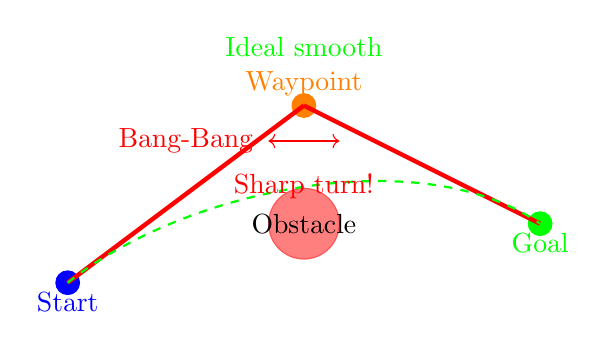
\begin{tikzpicture}[scale=1.5]
    % Robot positions
    \filldraw[blue] (0,0) circle (0.1) node[below] {Start};
    \filldraw[orange] (2,1.5) circle (0.1) node[above] {Waypoint};
    \filldraw[green] (4,0.5) circle (0.1) node[below] {Goal};
    
    % Obstacle
    \filldraw[red, opacity=0.5] (2,0.5) circle (0.3);
    \node at (2,0.5) {Obstacle};
    
    % Pure Bang-Bang (sharp)
    \draw[red, ultra thick] (0,0) -- (2,1.5);
    \draw[red, ultra thick] (2,1.5) -- (4,0.5);
    \node[red] at (1,1.2) {Bang-Bang};
    
    % Smooth curve
    \draw[green, thick, dashed] (0,0) .. controls (1,0.8) and (3,1.2) .. (4,0.5);
    \node[green] at (2,2) {Ideal smooth};
    
    % Sharp corner annotation
    \draw[<->, red] (1.7,1.2) -- (2.3,1.2);
    \node[red, below] at (2,1) {Sharp turn!};
\end{tikzpicture}
\caption{Bang-Bang creates sharp corners at waypoints}
\end{figure}

At each waypoint, Bang-Bang trajectory has these problems:
\begin{itemize}
    \item \textbf{Velocity Discontinuity:} The robot must completely change direction
    \item \textbf{Zero Velocity at Corners:} Robot often needs to stop to change direction
    \item \textbf{Time Loss:} Deceleration to zero and re-acceleration wastes time
    \item \textbf{Mechanical Stress:} Sharp changes stress motors and wheels
\end{itemize}

\subsection{Sumatra's Solution: Trajectory Chaining with Velocity Continuity}

Sumatra solves this problem through a clever technique called \textbf{trajectory chaining with early switching}:

\begin{algorithm}
\caption{Sumatra's Smooth Path Generation}
\begin{algorithmic}
\STATE \textbf{Key Insight:} Don't wait to reach the waypoint before planning the next segment!

\STATE \textbf{Step 1: Generate Initial Trajectory}
\STATE Create Bang-Bang trajectory toward sub-destination

\STATE \textbf{Step 2: Early Path Switching}
\FOR{$t = 0.2s, 0.4s, 0.6s, ...$ along trajectory}
    \STATE Calculate robot state at time $t$:
    \STATE $pos_t = trajectory.getPosition(t)$
    \STATE $vel_t = trajectory.getVelocity(t)$ \COMMENT{Non-zero velocity!}
    
    \STATE \textbf{Step 3: Append New Trajectory}
    \STATE Generate new Bang-Bang from $(pos_t, vel_t)$ to goal
    \STATE This preserves velocity continuity!
    
    \IF{Combined path is collision-free}
        \STATE \textbf{Return} smooth combined trajectory
    \ENDIF
\ENDFOR
\end{algorithmic}
\end{algorithm}

\section{How Sumatra Achieves Smoothness: The Complete Picture}

\subsection{Your Understanding vs Reality}

\textbf{Your Understanding:} "When there's an obstacle, regenerate trajectory from sub-destination points that are very close to the robot's current position."

\textbf{The Reality:} Not quite! Sumatra does something cleverer:

\begin{enumerate}
    \item Generate trajectory to a \textbf{far away} sub-destination (around the obstacle)
    \item \textbf{Don't go all the way there!}
    \item Instead, try switching to the goal at multiple points along this trajectory
    \item Switch at the \textbf{earliest safe point} that avoids collision
\end{enumerate}

\subsection{The Mathematical Foundation}

Let's denote:
\begin{itemize}
    \item $\mathbf{p}_0$ = Robot's current position
    \item $\mathbf{v}_0$ = Robot's current velocity  
    \item $\mathbf{p}_g$ = Goal position
    \item $\mathbf{p}_s$ = Sub-destination (waypoint around obstacle)
    \item $\gamma_1(t)$ = Trajectory from $\mathbf{p}_0$ to $\mathbf{p}_s$
    \item $\gamma_2(t)$ = Trajectory from switching point to $\mathbf{p}_g$
\end{itemize}

The key equation for smoothness at switching time $t_s$:

\begin{equation}
\boxed{\mathbf{v}_{\gamma_2}(0) = \mathbf{v}_{\gamma_1}(t_s)}
\end{equation}

This ensures velocity continuity! The second trajectory starts with the exact velocity the first trajectory had at the switching point.

\subsection{The Algorithm in Detail}

\begin{algorithm}
\caption{Sumatra's Smooth Path Generation (Corrected)}
\begin{algorithmic}
\STATE \textbf{Input:} Robot position $\mathbf{p}_0$, velocity $\mathbf{v}_0$, goal $\mathbf{p}_g$, obstacle

\STATE \textbf{Step 1: Direct Path Check}
\STATE $\gamma_{direct} \gets$ BangBang($\mathbf{p}_0$, $\mathbf{v}_0$, $\mathbf{p}_g$)
\IF{no collision on $\gamma_{direct}$}
    \STATE \textbf{return} $\gamma_{direct}$
\ENDIF

\STATE \textbf{Step 2: Generate Sub-destinations Around Obstacle}
\FOR{each sub-destination $\mathbf{p}_s$ around obstacle}
    \STATE $\gamma_1 \gets$ BangBang($\mathbf{p}_0$, $\mathbf{v}_0$, $\mathbf{p}_s$)
    
    \STATE \textbf{Step 3: Try Early Switching (KEY STEP!)}
    \FOR{$t_s = 0.2s, 0.4s, 0.6s, ...$ along $\gamma_1$}
        \STATE \COMMENT{Get state at switching time}
        \STATE $\mathbf{p}_{switch} = \gamma_1.position(t_s)$
        \STATE $\mathbf{v}_{switch} = \gamma_1.velocity(t_s)$ \COMMENT{Non-zero!}
        
        \STATE \COMMENT{Generate new trajectory from switch point}
        \STATE $\gamma_2 \gets$ BangBang($\mathbf{p}_{switch}$, $\mathbf{v}_{switch}$, $\mathbf{p}_g$)
        
        \STATE \COMMENT{Combine trajectories}
        \STATE $\gamma_{combined} = \gamma_1[0, t_s] \oplus \gamma_2$
        
        \IF{no collision on $\gamma_{combined}$}
            \STATE \textbf{return} $\gamma_{combined}$
        \ENDIF
    \ENDFOR
\ENDFOR
\end{algorithmic}
\end{algorithm}

\subsection{Why This Creates Smooth Paths: Mathematical Analysis}

The smoothness comes from the velocity matching at the switching point. Let's analyze the jerk (rate of change of acceleration):

\begin{figure}[H]
\centering
\begin{tikzpicture}[scale=2]
    % Coordinate axes
    \draw[->] (0,0) -- (4,0) node[right] {Time $t$};
    \draw[->] (0,0) -- (0,2.5) node[above] {Velocity $v$};
    
    % Trajectory 1 (to sub-destination)
    \draw[thick, blue] (0,0.3) -- (1,1.3) -- (2,1.3);
    \node[blue] at (1.5,1.5) {$\gamma_1$ to $\mathbf{p}_s$};
    
    % Switching points
    \foreach \t/\v in {0.4/0.7, 0.6/0.9, 0.8/1.1, 1.0/1.3} {
        \filldraw[orange] (\t,\v) circle (0.03);
    }
    
    % Selected switch at t=0.8
    \draw[thick, green, ->] (0.8,1.1) -- (2.5,0.2);
    \node[green] at (1.8,0.7) {$\gamma_2$ to goal};
    
    % Annotations
    \draw[dashed] (0.8,0) -- (0.8,1.1);
    \node[below] at (0.8,0) {$t_s = 0.8s$};
    \node[orange] at (0.6,0.5) {Try switch};
    
    % Velocity continuity
    \draw[<->, red] (0.75,1.15) -- (0.85,1.05);
    \node[red, right] at (1,1.1) {Same $v$!};
\end{tikzpicture}
\caption{Velocity continuity at switching point ensures smoothness}
\end{figure}

\textbf{Mathematical Proof of Reduced Jerk:}

Traditional approach (stop at waypoint):
\begin{align}
    \text{Jerk}_1 &= \frac{d a}{dt}\bigg|_{waypoint} = \infty \text{ (velocity discontinuity)}
\end{align}

Sumatra's approach (early switching):
\begin{align}
    \text{Jerk}_2 &= \frac{d a}{dt}\bigg|_{switch} = \frac{a_{\gamma_2}(0) - a_{\gamma_1}(t_s)}{\Delta t}
\end{align}

Since velocities match at the switch point:
\begin{align}
    v_{\gamma_2}(0) &= v_{\gamma_1}(t_s) \\
    \Rightarrow \text{Jerk}_2 &< \infty \text{ (finite jerk)}
\end{align}

\subsection{The Closer to Obstacle, The Smoother the Path}

You're partially correct! When the robot is close to an obstacle:

\begin{enumerate}
    \item \textbf{Shorter switch times:} Can switch earlier (e.g., at $t_s = 0.2s$ instead of $1.0s$)
    \item \textbf{Lower velocities:} Robot is often slower near obstacles
    \item \textbf{Smaller angle changes:} Direction change is more gradual
\end{enumerate}

\begin{figure}[H]
\centering
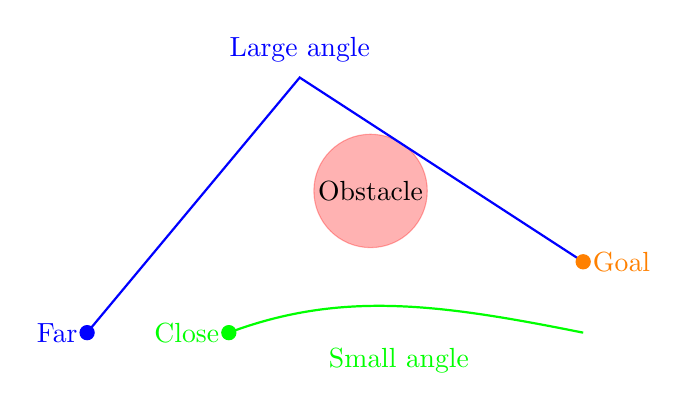
\begin{tikzpicture}[scale=1.8]
    % Obstacle
    \filldraw[red, opacity=0.3] (2,1) circle (0.4);
    \node at (2,1) {Obstacle};
    
    % Far from obstacle
    \begin{scope}[shift={(0,0)}]
        \filldraw[blue] (0,0) circle (0.05) node[left] {Far};
        \draw[blue, thick] (0,0) -- (1.5,1.8) -- (3.5,0.5);
        \node[blue] at (1.5,2) {Large angle};
    \end{scope}
    
    % Close to obstacle
    \begin{scope}[shift={(0,-0.5)}]
        \filldraw[green] (1,0.5) circle (0.05) node[left] {Close};
        \draw[green, thick] (1,0.5) .. controls (1.8,0.8) and (2.5,0.7) .. (3.5,0.5);
        \node[green] at (2.2,0.3) {Small angle};
    \end{scope}
    
    % Goal
    \filldraw[orange] (3.5,0.5) circle (0.05) node[right] {Goal};
\end{tikzpicture}
\caption{Closer to obstacle = Smaller direction changes = Smoother path}
\end{figure}

\subsection{Concrete Numerical Example}

Let's work through a real example with numbers:

\begin{figure}[H]
\centering
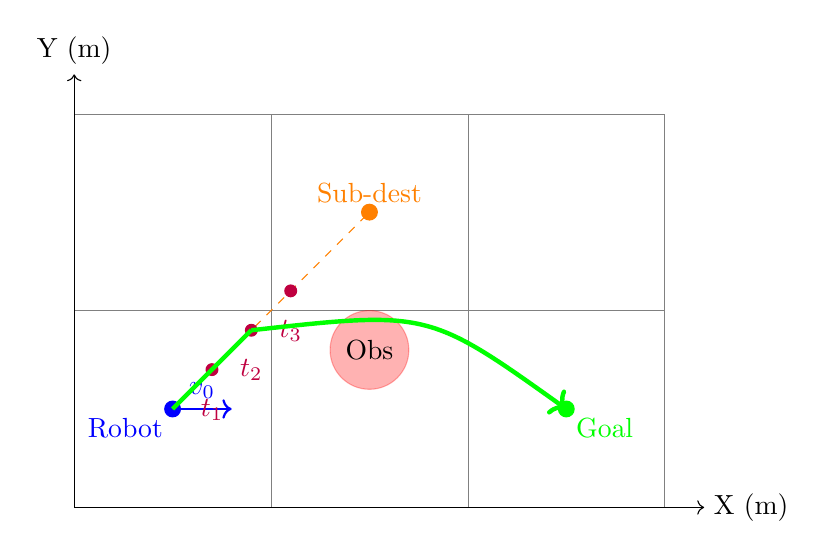
\begin{tikzpicture}[scale=2.5]
    % Grid
    \draw[gray, very thin] (0,0) grid (3,2);
    
    % Axes
    \draw[->] (0,0) -- (3.2,0) node[right] {X (m)};
    \draw[->] (0,0) -- (0,2.2) node[above] {Y (m)};
    
    % Robot start
    \filldraw[blue] (0.5,0.5) circle (0.04) node[below left] {Robot};
    \draw[->, blue, thick] (0.5,0.5) -- (0.8,0.5) node[midway, above] {$v_0$};
    
    % Obstacle
    \filldraw[red, opacity=0.3] (1.5,0.8) circle (0.2);
    \node at (1.5,0.8) {Obs};
    
    % Goal
    \filldraw[green] (2.5,0.5) circle (0.04) node[below right] {Goal};
    
    % Sub-destination
    \filldraw[orange] (1.5,1.5) circle (0.04) node[above] {Sub-dest};
    
    % Trajectory to sub-dest
    \draw[orange, dashed] (0.5,0.5) -- (1.5,1.5);
    
    % Switch points with times
    \foreach \t/\x/\y/\label in {0.2/0.7/0.7/$t_1$, 0.4/0.9/0.9/$t_2$, 0.6/1.1/1.1/$t_3$} {
        \filldraw[purple] (\x,\y) circle (0.03);
        \node[purple, below] at (\x,\y-0.1) {\label};
    }
    
    % Actual path (switches at t2)
    \draw[green, ultra thick] (0.5,0.5) -- (0.9,0.9);
    \draw[green, ultra thick, ->] (0.9,0.9) .. controls (1.8,1.0) .. (2.5,0.5);
\end{tikzpicture}
\caption{Numerical example of trajectory switching}
\end{figure}

\textbf{Given:}
\begin{itemize}
    \item Robot at $(0.5, 0.5)$ m with velocity $(0.3, 0)$ m/s
    \item Obstacle at $(1.5, 0.8)$ m with radius $0.2$ m
    \item Goal at $(2.5, 0.5)$ m
    \item Sub-destination at $(1.5, 1.5)$ m
\end{itemize}

\textbf{Step-by-step execution:}

\begin{enumerate}
    \item \textbf{Generate $\gamma_1$ to sub-destination:}
    \begin{itemize}
        \item Bang-Bang from $(0.5, 0.5)$ to $(1.5, 1.5)$
        \item Distance: $\sqrt{1^2 + 1^2} = 1.41$ m
        \item Estimated time: $\approx 1.8$ seconds
    \end{itemize}
    
    \item \textbf{Try switching at $t_1 = 0.2$ s:}
    \begin{itemize}
        \item Position: $(0.7, 0.7)$ m
        \item Velocity: $(0.5, 0.5)$ m/s (accelerating)
        \item Generate $\gamma_2$ from here to goal
        \item Check collision: COLLISION with obstacle! ❌
    \end{itemize}
    
    \item \textbf{Try switching at $t_2 = 0.4$ s:}
    \begin{itemize}
        \item Position: $(0.9, 0.9)$ m  
        \item Velocity: $(0.6, 0.6)$ m/s (still accelerating)
        \item Generate $\gamma_2$ from here to goal
        \item Check collision: NO COLLISION! ✓
        \item \textbf{This is our path!}
    \end{itemize}
    
    \item \textbf{Final trajectory:}
    \begin{itemize}
        \item Segment 1: $(0.5, 0.5) \to (0.9, 0.9)$ in $0.4$ s
        \item Segment 2: $(0.9, 0.9) \to (2.5, 0.5)$ starting with $\mathbf{v} = (0.6, 0.6)$ m/s
        \item Total time: $\approx 1.5$ s (faster than going to sub-destination!)
    \end{itemize}
\end{enumerate}

\textbf{Key Insight:} The robot never reaches the sub-destination! It switches early, maintaining momentum.

\subsection{Why Step Size of 0.2s Works Well}

The 0.2 second step size is carefully chosen:

\begin{table}[h]
\centering
\begin{tabular}{|l|c|p{6cm}|}
\hline
\textbf{Step Size} & \textbf{Value} & \textbf{Effect} \\
\hline
Too small (0.05s) & Bad & Too many checks, minimal path difference \\
\textbf{Just right (0.2s)} & \textbf{Good} & \textbf{Balance of smoothness and computation} \\
Too large (1.0s) & Bad & Might miss good switching opportunities \\
\hline
\end{tabular}
\caption{Effect of step size on path quality}
\end{table}

At robot speed of 1 m/s, 0.2s means checking every 20cm along the path - enough granularity to find smooth transitions without excessive computation.

\subsection{Visual Comparison: Traditional vs Sumatra Approach}

\begin{figure}[H]
\centering
\begin{subfigure}{0.45\textwidth}
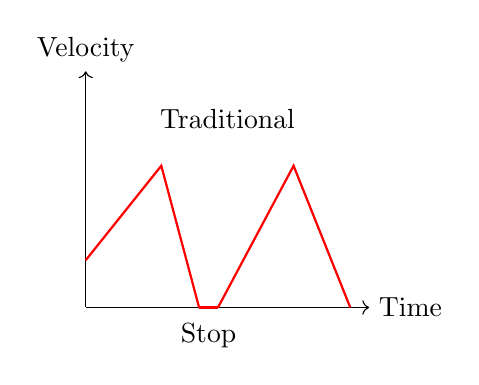
\begin{tikzpicture}[scale=1.2]
    % Traditional approach
    \draw[->] (0,0) -- (3,0) node[right] {Time};
    \draw[->] (0,0) -- (0,2.5) node[above] {Velocity};
    
    % First segment
    \draw[thick, red] (0,0.5) -- (0.8,1.5) -- (1.2,0);
    % Stop at waypoint
    \draw[thick, red] (1.2,0) -- (1.4,0);
    % Second segment
    \draw[thick, red] (1.4,0) -- (2.2,1.5) -- (2.8,0);
    
    \node at (1.3,-0.3) {Stop};
    \node at (1.5,2) {Traditional};
\end{tikzpicture}
\caption{Stop at waypoint}
\end{subfigure}
\hfill
\begin{subfigure}{0.45\textwidth}
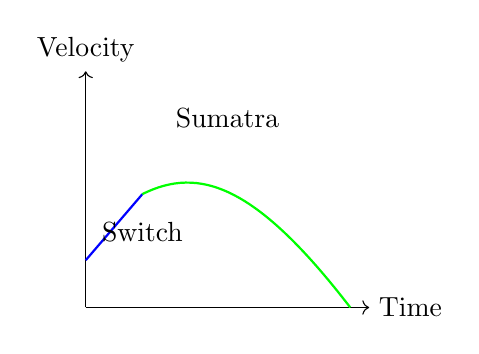
\begin{tikzpicture}[scale=1.2]
    % Sumatra approach
    \draw[->] (0,0) -- (3,0) node[right] {Time};
    \draw[->] (0,0) -- (0,2.5) node[above] {Velocity};
    
    % First segment (partial)
    \draw[thick, blue] (0,0.5) -- (0.6,1.2);
    % Smooth transition
    \draw[thick, green] (0.6,1.2) .. controls (1.2,1.5) and (1.8,1.3) .. (2.8,0);
    
    \node at (0.6,0.8) {Switch};
    \node at (1.5,2) {Sumatra};
\end{tikzpicture}
\caption{Switch before waypoint}
\end{subfigure}
\caption{Velocity profiles: Traditional vs Sumatra approach}
\end{figure}

\subsection{The Step-by-Step Algorithm}

Let's trace through a concrete example:

\begin{enumerate}
    \item \textbf{Initial State:}
    \begin{itemize}
        \item Robot at $(0, 0)$ with velocity $(0.5, 0)$ m/s
        \item Obstacle at $(2, 0)$
        \item Goal at $(4, 0)$
        \item Sub-destination at $(2, 2)$ (to avoid obstacle)
    \end{itemize}
    
    \item \textbf{Generate trajectory to sub-destination:}
    \begin{itemize}
        \item Bang-Bang trajectory from $(0,0)$ to $(2,2)$
        \item Total time: 2.5 seconds
    \end{itemize}
    
    \item \textbf{Try early switching at $t = 0.4s$:}
    \begin{itemize}
        \item Position at $t=0.4s$: $(0.35, 0.15)$
        \item Velocity at $t=0.4s$: $(0.7, 0.3)$ m/s (moving!)
        \item Generate new trajectory from this state to goal $(4, 0)$
        \item Check if combined path avoids obstacle
    \end{itemize}
    
    \item \textbf{Result:}
    \begin{itemize}
        \item Smooth curved path that never stops
        \item Maintains momentum throughout
        \item Reaches goal faster than stop-and-go approach
    \end{itemize}
\end{enumerate}

\subsection{Why Early Switching Works}

\begin{figure}[H]
\centering
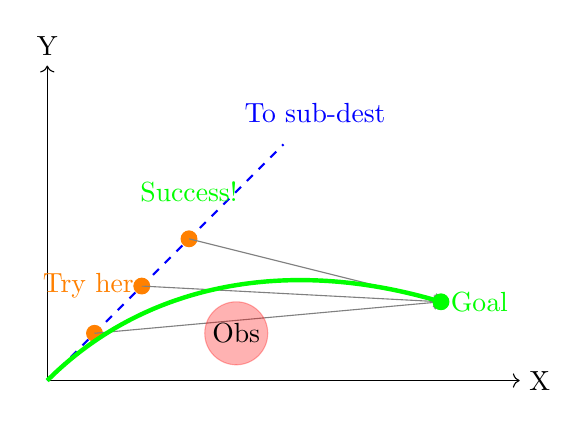
\begin{tikzpicture}[scale=2]
    % Coordinate system
    \draw[->] (0,0) -- (3,0) node[right] {X};
    \draw[->] (0,0) -- (0,2) node[above] {Y};
    
    % Original trajectory to sub-dest
    \draw[blue, dashed, thick] (0,0) -- (1.5,1.5);
    \node[blue] at (1.7,1.7) {To sub-dest};
    
    % Switch points
    \foreach \t/\x/\y in {0.2/0.3/0.3, 0.4/0.6/0.6, 0.6/0.9/0.9} {
        \filldraw[orange] (\x,\y) circle (0.05);
        \draw[gray, ->] (\x,\y) -- (2.5,0.5);
    }
    
    % Selected path
    \draw[green, ultra thick] (0,0) .. controls (0.6,0.6) and (1.5,0.8) .. (2.5,0.5);
    
    % Obstacle
    \filldraw[red, opacity=0.3] (1.2,0.3) circle (0.2);
    \node at (1.2,0.3) {Obs};
    
    % Goal
    \filldraw[green] (2.5,0.5) circle (0.05) node[right] {Goal};
    
    % Annotations
    \node[orange] at (0.3,0.6) {Try here};
    \node[green] at (0.9,1.2) {Success!};
\end{tikzpicture}
\caption{Multiple switch points tested for smoothest path}
\end{figure}

The algorithm tests multiple "switch points" along the initial trajectory:
\begin{itemize}
    \item Earlier switches = Smoother curves (larger turning radius)
    \item Later switches = Closer to sub-destination (better obstacle clearance)
    \item Sweet spot: Balance between smoothness and safety
\end{itemize}

\section{Obstacle Avoidance Strategy}

\subsection{The Path-Finding Algorithm}

Sumatra doesn't use traditional path-finding algorithms like A* or RRT*. Instead, it uses a clever approach:

\begin{algorithm}
\caption{Sumatra's Obstacle Avoidance}
\begin{algorithmic}
\STATE \textbf{Step 1: Try Direct Path}
\STATE Generate Bang-Bang trajectory directly to goal
\IF{No collision detected}
    \STATE \textbf{Return} direct trajectory
\ENDIF

\STATE \textbf{Step 2: Generate Sub-Destinations}
\FOR{each obstacle near the path}
    \STATE Generate random points around obstacle
    \STATE Points are at different angles and distances
\ENDFOR

\STATE \textbf{Step 3: Try Each Sub-Destination}
\FOR{each sub-destination}
    \STATE Generate trajectory to sub-destination
    \IF{No collision to sub-destination}
        \STATE Check if path from sub-destination to goal is clear
        \IF{Path is clear}
            \STATE \textbf{Return} combined trajectory
        \ENDIF
    \ENDIF
\ENDFOR

\STATE \textbf{Step 4: Choose Best Partial Path}
\STATE Return the path that gets closest to goal
\end{algorithmic}
\end{algorithm}

\subsection{Sub-Destination Generation}

Sub-destinations are generated using these parameters:
\begin{itemize}
    \item \textbf{Angle Range:} $20° - 140°$ from direct path
    \item \textbf{Distance Scale:} $0.5 - 1.5$ times the distance to goal
    \item \textbf{Number of Points:} Typically 5 random points
\end{itemize}

\begin{figure}[H]
\centering
\begin{tikzpicture}[scale=2]
    % Robot and goal
    \filldraw[blue] (0,0) circle (0.1) node[below] {Robot};
    \filldraw[green] (4,2) circle (0.1) node[above] {Goal};
    
    % Obstacle
    \filldraw[red, opacity=0.5] (2,1) circle (0.3);
    \node at (2,1) {Obstacle};
    
    % Direct path (blocked)
    \draw[red, dashed, thick] (0,0) -- (4,2);
    
    % Sub-destinations
    \foreach \angle/\dist in {30/1.2, 60/0.8, -30/1.0, -60/1.3, 90/0.7} {
        \filldraw[orange] ($(0,0) + (\angle:{\dist*2.5})$) circle (0.05);
    }
    
    % Example avoidance path
    \draw[green, thick] (0,0) .. controls (1,1.5) and (3,2.5) .. (4,2);
    
    % Legend
    \node[orange] at (1.5,2.5) {Sub-destinations};
\end{tikzpicture}
\caption{Sub-Destination Generation Around Obstacle}
\end{figure}

\section{Collision Detection}

\subsection{Time-Based Collision Checking}

Instead of checking the entire trajectory at once, Sumatra checks collisions at discrete time steps:

\begin{algorithm}
\caption{Collision Detection Algorithm}
\begin{algorithmic}
\STATE $\Delta t = 0.01$ seconds \COMMENT{10ms time step}
\FOR{$t = 0$ to $t_{total}$ step $\Delta t$}
    \STATE $pos_{robot} = trajectory.getPosition(t)$
    \FOR{each obstacle}
        \IF{obstacle is moving}
            \STATE $pos_{obstacle} = obstacle.position + obstacle.velocity \cdot t$
        \ELSE
            \STATE $pos_{obstacle} = obstacle.position$
        \ENDIF
        \STATE $distance = ||pos_{robot} - pos_{obstacle}||$
        \IF{$distance < radius_{robot} + radius_{obstacle} + margin$}
            \STATE \textbf{Return} "Collision at time $t$"
        \ENDIF
    \ENDFOR
\ENDFOR
\STATE \textbf{Return} "No collision"
\end{algorithmic}
\end{algorithm}

\subsection{Dynamic Margin}

The collision margin is adjusted based on robot velocity:
\begin{equation}
    margin = margin_{static} + k \cdot ||v_{robot}||
\end{equation}

This gives the robot more clearance when moving fast!

\section{Implementation Details}

\subsection{Trajectory Parts Structure}

Each 1D trajectory consists of up to 3 parts:

\begin{lstlisting}[language=Java, caption=Trajectory Part Structure]
class BBTrajectoryPart {
    float tEnd;    // End time of this part
    float acc;     // Acceleration during this part
    float v0;      // Initial velocity
    float s0;      // Initial position
}
\end{lstlisting}

\subsection{Position Calculation}

At any time $t$, the position is calculated by:
\begin{enumerate}
    \item Find which part contains time $t$
    \item Calculate time within that part: $t_{local} = t - t_{part\_start}$
    \item Apply kinematic equation: $s = s_0 + v_0 \cdot t_{local} + \frac{1}{2} a \cdot t_{local}^2$
\end{enumerate}

\subsection{Memory Efficiency}

Sumatra pre-allocates arrays for trajectory parts:
\begin{itemize}
    \item Maximum 3 parts per 1D trajectory
    \item No dynamic memory allocation during trajectory generation
    \item Fast computation suitable for real-time control
\end{itemize}

\section{Smoothness Guarantees and Trade-offs}

\subsection{What Sumatra Guarantees}

\begin{itemize}
    \item \textbf{C0 Continuity (Position):} Position is always continuous
    \item \textbf{C1 Continuity (Velocity):} Velocity is continuous at switch points
    \item \textbf{NOT C2 Continuous (Acceleration):} Acceleration can jump at switch points
\end{itemize}

\begin{figure}[H]
\centering
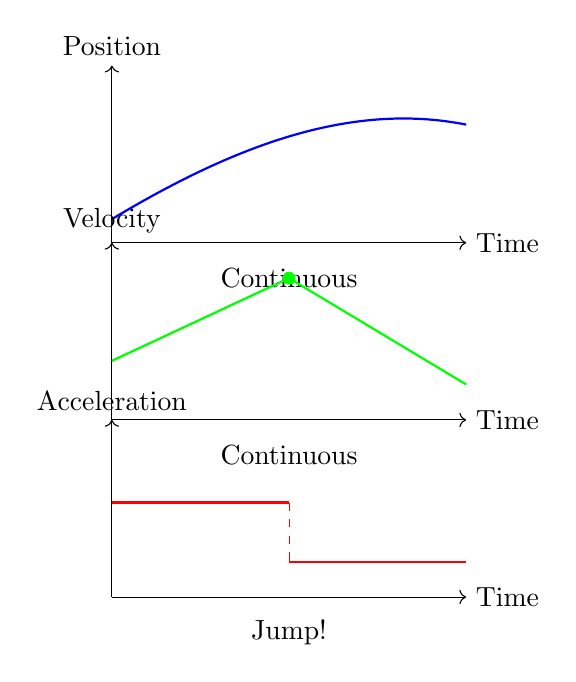
\begin{tikzpicture}[scale=1.5]
    % Position continuity
    \begin{scope}[shift={(0,3)}]
        \draw[->] (0,0) -- (3,0) node[right] {Time};
        \draw[->] (0,0) -- (0,1.5) node[above] {Position};
        \draw[thick, blue] (0,0.2) .. controls (1,0.8) and (2,1.2) .. (3,1.0);
        \node at (1.5,-0.3) {Continuous};
    \end{scope}
    
    % Velocity continuity
    \begin{scope}[shift={(0,1.5)}]
        \draw[->] (0,0) -- (3,0) node[right] {Time};
        \draw[->] (0,0) -- (0,1.5) node[above] {Velocity};
        \draw[thick, green] (0,0.5) -- (1.5,1.2);
        \draw[thick, green] (1.5,1.2) -- (3,0.3);
        \filldraw[green] (1.5,1.2) circle (0.05);
        \node at (1.5,-0.3) {Continuous};
    \end{scope}
    
    % Acceleration discontinuity
    \begin{scope}
        \draw[->] (0,0) -- (3,0) node[right] {Time};
        \draw[->] (0,0) -- (0,1.5) node[above] {Acceleration};
        \draw[thick, red] (0,0.8) -- (1.5,0.8);
        \draw[thick, red] (1.5,0.3) -- (3,0.3);
        \draw[dashed, red] (1.5,0.8) -- (1.5,0.3);
        \node at (1.5,-0.3) {Jump!};
    \end{scope}
\end{tikzpicture}
\caption{Continuity properties of Sumatra's trajectories}
\end{figure}

\subsection{Trade-offs: Smoothness vs Time-Optimality}

\begin{table}[h]
\centering
\begin{tabular}{|l|c|c|c|}
\hline
\textbf{Approach} & \textbf{Time to Goal} & \textbf{Smoothness} & \textbf{Computation} \\
\hline
Pure Bang-Bang (stop at waypoints) & Slow & Jerky & Fast \\
Early switching (Sumatra) & Fast & Smooth velocity & Fast \\
Spline-based (B-Spline, Bezier) & Slower & Very smooth & Slower \\
Optimization-based (MPC) & Variable & Configurable & Slow \\
\hline
\end{tabular}
\caption{Comparison of different trajectory planning approaches}
\end{table}

\subsection{When Sumatra's Approach Excels}

Sumatra's method works best when:
\begin{enumerate}
    \item \textbf{Obstacles are sparse:} Fewer waypoints needed
    \item \textbf{Speed matters:} Time-optimal between waypoints
    \item \textbf{Real-time constraints:} Fast computation required
    \item \textbf{Dynamic environment:} Can quickly replan
\end{enumerate}

\subsection{When Other Methods Might Be Better}

Consider alternatives when:
\begin{enumerate}
    \item \textbf{Dense obstacles:} Many waypoints create jerky motion
    \item \textbf{Precision over speed:} Exact path following required
    \item \textbf{Smooth acceleration needed:} For delicate tasks
    \item \textbf{Energy efficiency matters:} Bang-Bang uses maximum power
\end{enumerate}

\section{Performance Optimization}

\subsection{Binary Search for Synchronization}

The alpha-synchronization uses binary search with fixed iterations:
\begin{itemize}
    \item Start with $\alpha = \pi/4$ (45°)
    \item Initial increment: $\Delta\alpha = \pi/8$
    \item Halve increment each iteration: $\Delta\alpha = \Delta\alpha / 2$
    \item Stop when $\Delta\alpha < 10^{-7}$ or time difference $< 1ms$
\end{itemize}

\subsection{Fast Math Operations}

Sumatra uses optimized math libraries:
\begin{itemize}
    \item \texttt{FastMath.sinAndCos()}: Computes both sin and cos in one operation
    \item Fixed-point arithmetic where possible
    \item Pre-computed constants
\end{itemize}

\section{Advantages of Bang-Bang Control}

\subsection{Time Optimality}

\textbf{Theorem (Pontryagin's Maximum Principle):}
For a system with bounded control (limited acceleration), the time-optimal trajectory uses maximum control effort at all times.

\textbf{Simple Explanation:}
To get somewhere fastest with limited acceleration, you should always be either:
\begin{itemize}
    \item Accelerating at maximum
    \item Decelerating at maximum
    \item Cruising at maximum speed
\end{itemize}
Never use partial acceleration!

\subsection{Computational Efficiency}

\begin{itemize}
    \item \textbf{Analytical Solution:} No iterative optimization needed
    \item \textbf{Constant Time:} $O(1)$ trajectory generation
    \item \textbf{Predictable:} Easy to verify and debug
    \item \textbf{No Local Minima:} Always finds the optimal solution
\end{itemize}

\subsection{Comparison with Other Methods}

\begin{center}
\begin{tabular}{|l|c|c|c|c|}
\hline
\textbf{Method} & \textbf{Time-Optimal} & \textbf{Smooth} & \textbf{Fast} & \textbf{Simple} \\
\hline
Bang-Bang & \checkmark & $\times$ & \checkmark & \checkmark \\
B-Spline & $\times$ & \checkmark & \checkmark & $\times$ \\
RRT* & $\times$ & $\times$ & $\times$ & $\times$ \\
A* & $\times$ & $\times$ & Medium & \checkmark \\
\hline
\end{tabular}
\end{center}

\section{Real-World Considerations}

\subsection{Motor Response}

Real motors can't change acceleration instantly. Sumatra handles this by:
\begin{itemize}
    \item Using slightly lower maximum acceleration than physical limit
    \item Adding small time margins at trajectory switches
    \item Low-level motor controllers handle smoothing
\end{itemize}

\subsection{Sensor Noise}

Position sensors have noise. The system handles this by:
\begin{itemize}
    \item Kalman filtering for state estimation
    \item Replanning trajectories frequently (every 10-20ms)
    \item Using feedback control on top of feedforward trajectory
\end{itemize}

\subsection{Multi-Robot Coordination}

When multiple robots are moving:
\begin{itemize}
    \item Each robot treats others as moving obstacles
    \item Priority system prevents deadlocks
    \item Robots with ball have higher priority
\end{itemize}

\section{Example: Complete Trajectory Calculation}

Let's work through a concrete example:

\textbf{Given:}
\begin{itemize}
    \item Start position: $(0, 0)$ meters
    \item Goal position: $(2, 1)$ meters
    \item Initial velocity: $(0.5, 0)$ m/s
    \item Max velocity: $2$ m/s
    \item Max acceleration: $3$ m/s²
\end{itemize}

\textbf{Step 1: Initial Trajectories}
\begin{itemize}
    \item X-axis: $0 \to 2$m with $v_0 = 0.5$ m/s
    \item Y-axis: $0 \to 1$m with $v_0 = 0$ m/s
\end{itemize}

\textbf{Step 2: Alpha Synchronization}
\begin{enumerate}
    \item Try $\alpha = 45°$:
    \begin{itemize}
        \item $v_{max,x} = 2 \cdot \cos(45°) = 1.414$ m/s
        \item $v_{max,y} = 2 \cdot \sin(45°) = 1.414$ m/s
        \item $t_x \approx 1.5$ seconds
        \item $t_y \approx 1.0$ seconds
    \end{itemize}
    
    \item Since $t_x > t_y$, decrease $\alpha$ to $45° - 22.5° = 22.5°$
    
    \item Continue binary search until synchronized...
    
    \item Final: $\alpha \approx 30°$, both axes finish at $t = 1.3$ seconds
\end{enumerate}

\textbf{Step 3: Result}
\begin{itemize}
    \item Total time: 1.3 seconds
    \item Peak velocity: $(1.73, 1.0)$ m/s
    \item Path: Nearly straight line with slight curve due to initial velocity
\end{itemize}

\section{Code Structure Summary}

\subsection{Class Hierarchy}

\begin{center}
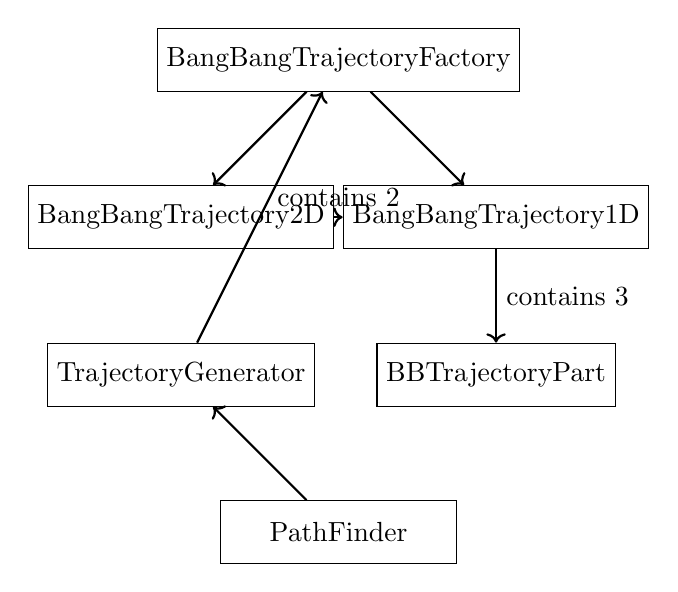
\begin{tikzpicture}[
    box/.style={rectangle, draw, minimum width=3cm, minimum height=0.8cm},
    arrow/.style={->, thick}
]
    % Classes
    \node[box] (factory) at (0,4) {BangBangTrajectoryFactory};
    \node[box] (traj2d) at (-2,2) {BangBangTrajectory2D};
    \node[box] (traj1d) at (2,2) {BangBangTrajectory1D};
    \node[box] (part) at (2,0) {BBTrajectoryPart};
    \node[box] (gen) at (-2,0) {TrajectoryGenerator};
    \node[box] (path) at (0,-2) {PathFinder};
    
    % Connections
    \draw[arrow] (factory) -- (traj2d);
    \draw[arrow] (factory) -- (traj1d);
    \draw[arrow] (traj2d) -- (traj1d) node[midway, above] {contains 2};
    \draw[arrow] (traj1d) -- (part) node[midway, right] {contains 3};
    \draw[arrow] (gen) -- (factory);
    \draw[arrow] (path) -- (gen);
\end{tikzpicture}
\end{center}

\subsection{Key Methods}

\begin{itemize}
    \item \texttt{generate()}: Creates trajectory from parameters
    \item \texttt{getPosition(t)}: Returns position at time $t$
    \item \texttt{getVelocity(t)}: Returns velocity at time $t$
    \item \texttt{checkCollision()}: Validates trajectory safety
    \item \texttt{append()}: Chains trajectories together
\end{itemize}

\section{Conclusion}

Sumatra's Bang-Bang trajectory planning system achieves:
\begin{itemize}
    \item \textbf{Time-optimal} motion (mathematically proven)
    \item \textbf{Real-time} performance (< 1ms computation)
    \item \textbf{Robust} obstacle avoidance
    \item \textbf{Simple} implementation
    \item \textbf{Predictable} behavior
\end{itemize}

The key insight is that for time-optimal control with bounded inputs, the optimal solution is always "all or nothing" - maximum acceleration, maximum deceleration, or cruising at maximum speed.

\section{Practical Implementation Tips}

\subsection{For Your Own Implementation}

\begin{enumerate}
    \item \textbf{Start Simple:} Implement 1D Bang-Bang first
    \item \textbf{Test Thoroughly:} Edge cases include:
    \begin{itemize}
        \item Zero distance (already at goal)
        \item Initial velocity exceeds max velocity
        \item Moving in wrong direction
    \end{itemize}
    \item \textbf{Add Safety Margins:} Real robots need:
    \begin{itemize}
        \item 10-20\% acceleration margin
        \item 5-10\% velocity margin
        \item Minimum trajectory duration (avoid oscillation)
    \end{itemize}
    \item \textbf{Optimize Later:} First make it work, then:
    \begin{itemize}
        \item Use lookup tables for trigonometry
        \item Pre-allocate memory
        \item Cache trajectory computations
    \end{itemize}
\end{enumerate}

\subsection{Common Pitfalls to Avoid}

\begin{itemize}
    \item \textbf{Floating Point Errors:} Use epsilon comparisons
    \item \textbf{Division by Zero:} Check for zero acceleration/velocity
    \item \textbf{Angle Wrapping:} Normalize angles to $[-\pi, \pi]$
    \item \textbf{Unit Confusion:} Be consistent (m/s vs mm/s)
\end{itemize}

\section{Code Integration Example}

Here's how to integrate the Bang-Bang trajectory planner in your robot control system:

\subsection{Basic Setup}
\begin{lstlisting}[language=C++, caption=Setting up the planner]
// In RobotManager or similar class
BangBangTrajectoryPlanner planner;

// Set conservative limits for safety
planner.SetLimits(0.8, 2.0);  // 0.8 m/s max vel, 2 m/s^2 acc
planner.SetFeedbackGains(2.0, 0.5);  // Position and velocity gains

// Add obstacles (other robots, ball, etc.)
planner.ClearObstacles();
for (const auto& robot : other_robots) {
    planner.AddObstacle(robot.position, 0.2);  // 200mm radius
}
\end{lstlisting}

\subsection{Path Following}
\begin{lstlisting}[language=C++, caption=Following the trajectory]
// Generate path to target
planner.GeneratePath(current_pos, current_vel, 
                     target_pos, target_orientation);

// In control loop (running at ~100 Hz)
void ControlUpdate(double dt) {
    // Get command from planner
    Eigen::Vector3d cmd = planner.GetVelocityCommand(
        current_pos, current_vel, dt);
    
    // cmd contains [vx, vy, omega] in body frame
    double vx = cmd[0];
    double vy = cmd[1]; 
    double omega = cmd[2];
    
    // Send to robot motors
    SendVelocityToRobot(vx, vy, omega);
}
\end{lstlisting}

\subsection{Handling Multiple Waypoints}
\begin{lstlisting}[language=C++, caption=Multi-waypoint navigation]
std::vector<Eigen::Vector3d> waypoints = {
    {-1.0, -0.5, 0.0},    // Position and orientation
    {1.0, -0.5, M_PI/2},
    {1.0, 0.5, M_PI},
    {-1.0, 0.5, -M_PI/2}
};

size_t current_waypoint = 0;

void UpdateNavigation() {
    // Check if reached current waypoint
    double distance = (current_pos - waypoints[current_waypoint])
                      .head<2>().norm();
    
    if (distance < 0.05) {  // 50mm threshold
        current_waypoint++;
        if (current_waypoint < waypoints.size()) {
            // Plan to next waypoint
            planner.GeneratePath(current_pos, current_vel,
                waypoints[current_waypoint].head<2>(),
                waypoints[current_waypoint][2]);
        }
    }
}
\end{lstlisting}

\section{Tuning Guide}

\subsection{Velocity and Acceleration Limits}
\begin{itemize}
    \item \textbf{Start Low}: Begin with 50\% of robot's maximum capabilities
    \item \textbf{Gradual Increase}: Increase by 10\% increments while testing
    \item \textbf{Safety Margin}: Keep final values at 80-90\% of maximum
\end{itemize}

\subsection{Feedback Gains}
The feedback controller uses proportional control:
\begin{equation}
v_{cmd} = v_{planned} + k_p \cdot e_{pos} + k_v \cdot e_{vel}
\end{equation}

\begin{itemize}
    \item \textbf{Position Gain ($k_p$)}: Start at 2.0
        \begin{itemize}
            \item Too low: Robot lags behind trajectory
            \item Too high: Robot oscillates around path
        \end{itemize}
    \item \textbf{Velocity Gain ($k_v$)}: Start at 0.5
        \begin{itemize}
            \item Provides damping to reduce oscillations
            \item Usually 20-30\% of position gain
        \end{itemize}
\end{itemize}

\subsection{Common Issues and Solutions}

\begin{table}[h]
\centering
\begin{tabular}{|p{4cm}|p{7cm}|}
\hline
\textbf{Problem} & \textbf{Solution} \\
\hline
Robot overshoots corners & Reduce max velocity or increase deceleration distance \\
\hline
Oscillation around path & Reduce position gain, increase velocity gain \\
\hline
Gets stuck near obstacles & Increase obstacle radius or add safety margin \\
\hline
Jerky movement & Reduce acceleration limit or increase control loop rate \\
\hline
Path replanning too frequent & Add hysteresis to obstacle detection \\
\hline
\end{tabular}
\caption{Common trajectory tracking issues and solutions}
\end{table}

\section{Testing Strategy}

\subsection{Unit Tests}
\begin{enumerate}
    \item \textbf{Straight Line}: Test basic trajectory generation
    \item \textbf{90° Turn}: Verify corner handling  
    \item \textbf{Stop from Speed}: Test deceleration profile
    \item \textbf{Obstacle Avoidance}: Single static obstacle
\end{enumerate}

\subsection{Integration Tests}
\begin{enumerate}
    \item \textbf{Square Path}: Four 90° turns
    \item \textbf{Figure-8}: Smooth curves and direction changes
    \item \textbf{Dynamic Obstacles}: Moving robots
    \item \textbf{Narrow Passages}: Test precise navigation
\end{enumerate}

\subsection{Performance Metrics}
\begin{itemize}
    \item \textbf{Tracking Error}: RMS distance from planned path (target: < 50mm)
    \item \textbf{Completion Time}: Time to reach destination
    \item \textbf{Smoothness}: Acceleration changes per second
    \item \textbf{Safety}: Minimum distance to obstacles maintained
\end{itemize}

\appendix

\section{Mathematical Proofs}

\subsection{Proof of Time Optimality}

\textbf{Claim:} Bang-Bang control minimizes travel time for bounded acceleration systems.

\textbf{Proof (Intuitive):}
Consider any trajectory that doesn't use maximum acceleration. We can always improve it by:
\begin{enumerate}
    \item Increasing acceleration where it's not maximal
    \item This reaches target velocity sooner
    \item Thus reaches target position sooner
    \item Therefore, non-maximal acceleration is never optimal
\end{enumerate}

\subsection{Triangular vs Trapezoidal Decision}

\textbf{Question:} When to use triangular vs trapezoidal profile?

\textbf{Answer:} Calculate the peak velocity if we never cruise:
\begin{equation}
    v_{peak} = \sqrt{2 \cdot a_{max} \cdot d}
\end{equation}

If $v_{peak} < v_{max}$: Use triangular\\
If $v_{peak} \geq v_{max}$: Use trapezoidal

\section{Reference Equations}

\subsection{Triangular Profile}
\begin{align}
    t_1 &= \sqrt{\frac{2d}{a_{max}}} \\
    v_{peak} &= a_{max} \cdot t_1 \\
    t_{total} &= 2 \cdot t_1
\end{align}

\subsection{Trapezoidal Profile}
\begin{align}
    t_1 &= \frac{v_{max}}{a_{max}} \\
    d_1 &= \frac{1}{2} a_{max} \cdot t_1^2 \\
    d_2 &= d - 2 \cdot d_1 \\
    t_2 &= \frac{d_2}{v_{max}} \\
    t_{total} &= 2 \cdot t_1 + t_2
\end{align}

\section{Glossary}

\begin{itemize}
    \item \textbf{Bang-Bang Control:} Control strategy using only maximum or minimum control effort
    \item \textbf{Trajectory:} The path and timing of motion from start to goal
    \item \textbf{Profile:} The shape of velocity over time (triangular, trapezoidal)
    \item \textbf{Synchronization:} Making X and Y motions finish simultaneously
    \item \textbf{Sub-destination:} Intermediate waypoint to avoid obstacles
    \item \textbf{Time-optimal:} Achieving goal in minimum possible time
    \item \textbf{SSL:} Small Size League (RoboCup robot soccer)
    \item \textbf{Feedforward:} Control based on planned trajectory
    \item \textbf{Feedback:} Control based on error correction
\end{itemize}

\end{document}